\documentclass[a4paper,8pt]{beamer}
\mode<presentation>
{
  \usetheme{Boadilla}
  \setbeamercovered{invisible}
}

% --- Official UCSF Color Palette ---
\definecolor{ucsfNavy}{RGB}{5, 32, 73}
\definecolor{ucsfBlueGray}{RGB}{80, 99, 128}
\definecolor{ucsfDarkGray}{RGB}{135, 141, 150}
\definecolor{ucsfCoolGray}{RGB}{180, 185, 191}
\definecolor{ucsfGray}{RGB}{209, 211, 211}
\definecolor{ucsfLightGray}{RGB}{225, 227, 230}
\definecolor{ucsfOffWhite}{RGB}{242, 243, 244}

% --- Apply UCSF Colors to Your Working Theme ---
\setbeamercolor*{palette secondary}{use=structure,fg=white,bg=ucsfBlueGray}
\setbeamercolor*{palette tertiary}{use=structure,fg=white,bg=ucsfNavy}
\setbeamercolor*{structure}{fg=ucsfNavy}
\setbeamercolor*{title}{fg=ucsfNavy}

% Block colors with UCSF palette
\setbeamercolor{block title}{bg=ucsfBlueGray, fg=white}
\setbeamercolor{block body}{bg=ucsfOffWhite, fg=black}
\setbeamercolor{block title example}{bg=ucsfCoolGray, fg=white}
\setbeamercolor{block body example}{bg=ucsfCoolGray!20, fg=black}
\setbeamercolor{block title alerted}{bg=ucsfNavy, fg=white}
\setbeamercolor{block body alerted}{bg=ucsfNavy!10, fg=black}

% Required packages
\usepackage[utf8]{inputenc}
% COMMENT OUT BIBLIOGRAPHY FOR NOW - uncomment when you have presentation.bib
%\usepackage[backend=bibtex,maxbibnames=3]{biblatex}
%\addbibresource{presentation.bib}
\usepackage{graphicx,bm,tabularx,booktabs,subcaption,hyperref}
\usepackage{verbatim,adjustbox}
\usepackage[most]{tcolorbox}
\usepackage{epsfig,amsmath,xcolor,listings,caption}
\usepackage{empheq}
\usepackage{pgfplots}
\pgfplotsset{compat=newest}
\usepackage{array} % For newcolumntype
\usepackage{tikz}
\usetikzlibrary{shapes, arrows, positioning}

% Your existing settings that work
\setbeamertemplate{footline}[frame number]
\usepackage{tikz}
\usetikzlibrary{arrows,calc}
\definecolor{myblue}{RGB}{5,32,73}  % This matches ucsfNavy
\newcommand\xsetpos{6}
\setbeamercovered{transparent}
\beamertemplatenavigationsymbolsempty
\definecolor{dgreen}{rgb}{0.,0.6,0.}
\newcolumntype{d}[1]{D{.}{\cdot}{#1}}

% Custom commands with UCSF colors
\newcommand{\highlight}[1]{\colorbox{ucsfGray!30}{#1}}
\newcommand{\important}[1]{{\color{ucsfNavy}\textbf{#1}}}
\newcommand{\itemPause}{\pause\item}

% Highlight boxes
\newtcolorbox{highlightbox}[1][]{
  enhanced,
  colback=ucsfOffWhite,
  colframe=ucsfBlueGray,
  boxrule=0.5pt,
  arc=2mm,
  #1
}

% COMMENT OUT LOGO FOR NOW - uncomment when you have the logo file
%\usepackage{pgf}
%\logo{\pgfputat{\pgfxy(0.15,8)}{\pgfbox[right,base]{
\includegraphics[height=1.25cm]{figures/ucsf-logo.pdf}}}}
%\newcommand{\nologo}{\setbeamertemplate{logo}{}}

% Document metadata
\title{Group meeting presentation}
\author[S. G. Balasubramani]{Sree Ganesh Balasubramani}
\institute[UCSF]{Echeverria \& {\v S}ali Groups \\ University of California, San Francisco}
\date{July 26, 2025}

% Section transitions
\AtBeginSection[]
{
  \begin{frame}{Outline}
    \tableofcontents[currentsection]
  \end{frame}
}

\begin{document}

% Title slide
\maketitle

%----------------------------------------------------------------------------
\section{Trifunctional crosslinkers}
%----------------------------------------------------------------------------
\begin{frame}
  \frametitle{Structure of the trifunctional crosslinker}
  
  \begin{figure}
    \centering
    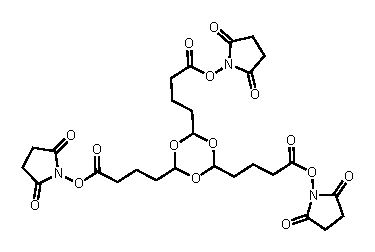
\includegraphics[width=0.4\textwidth]{figures/tri-linker.eps}
    \caption{Structure of TSTO MS cleavable crosslinker with a spacer arm length 
    of 14.0 \AA.}
  \end{figure}
  \begin{block}{}
    For comparison, the commonly used bifunctional crosslinker
  DSSO has a spacer arm length of 10.1 \AA.
    \end{block}
\end{frame}
%----------------------------------------------------------------------------
\begin{frame}
\frametitle{Riccardo's noise model for the crosslinking restraint}
\begin{equation}
p(o_n|X) \propto \frac{\alpha}{\beta}p(XL_n|X) + \frac{1 - \alpha}{1 - \beta}p(\bar{XL_n}|X)
\end{equation}
where 
\begin{equation}
\alpha = \frac{N^{obs, T}_{XL}}{N^{obs}_{XL}} \qquad \beta = \frac{N_{XL}}{N_{LP}}
\end{equation}
For trifunctional crosslinks, the $\beta$ parameter is modified to be 
\begin{equation}
\beta = \frac{N_{XL}^{tri}}{N_{LT}}
\end{equation}
where the number of lysine triplets $N_{LT}$ is 
given by $^{N_{lysines}}C_3 = \frac{N_{lysines}*(N_{lysines}-1)*(N_{lysines}-2)}{3!}$
\end{frame}
%----------------------------------------------------------------------------
\begin{frame}
    \frametitle{Trifunctional XL-MS data processing}
\begin{table}[h]
\centering
\small
\begin{tabular}{llrllr}
\toprule
Protein 1 & Residue 1 & Score 1 & Protein 2 & Residue 2 & Score 2 \\
\midrule
Rpn6  & K141 & 37.7 & Rpn6  & K325 & 22.9 \\
Rpn6  & K288 & 43.3 & Rpn6  & K304 & 51.2 \\
Rpn6  & K288 & 32.8 & Rpn6  & K304 & 45.6 \\
Rpn6  & K288 & 19.4 & Rpn6  & K304 & 48.4 \\
Rpn6  & K288 & 13.9 & Rpn6  & K304 & 43.9 \\
\bottomrule
\end{tabular}
\caption{Example bifunctional crosslinks (N = 3352 total).}
\end{table}
    \begin{table}[h]
\centering
\small
\begin{tabular}{llrllrllr}
\toprule
Protein 1 & Residue 1 & Score 1 & Protein 2 & Residue 2 & Score 2 & Protein 3 & Residue 3 & Score 3 \\
\midrule
Rpn5  & K294 & 12.6 & Rpn5  & K303 & 17.7 & Rpn9  & K132       & 25.6 \\
Rpn5  & K368 & 27.2 & Rpn5  & K376 & 17.4 & Rpn9  & K321;K329  & 31.1 \\
Rpn11 & K152 & 14.9 & Rpn11 & K223 & 19.2 & Rpn8  & K180       & 21.8 \\
Rpn11 & K264 & 40.1 & Rpn7  & K126 & 15.4 & Rpn7  & K163       & 20.6 \\
Rpn11 & K264 & 40.2 & Rpn7  & K126 & 17.4 & Rpn7  & K163       & 16.2 \\
\bottomrule
\end{tabular}
\caption{Example trifunctional crosslinks (N = 216 total).}
\end{table}
\end{frame}
%----------------------------------------------------------------------------
\begin{frame}
\frametitle{Normalizing the ID score}
% side by side figures
\begin{figure}
    \centering
    \begin{subfigure}[b]{0.45\textwidth}
        \centering
        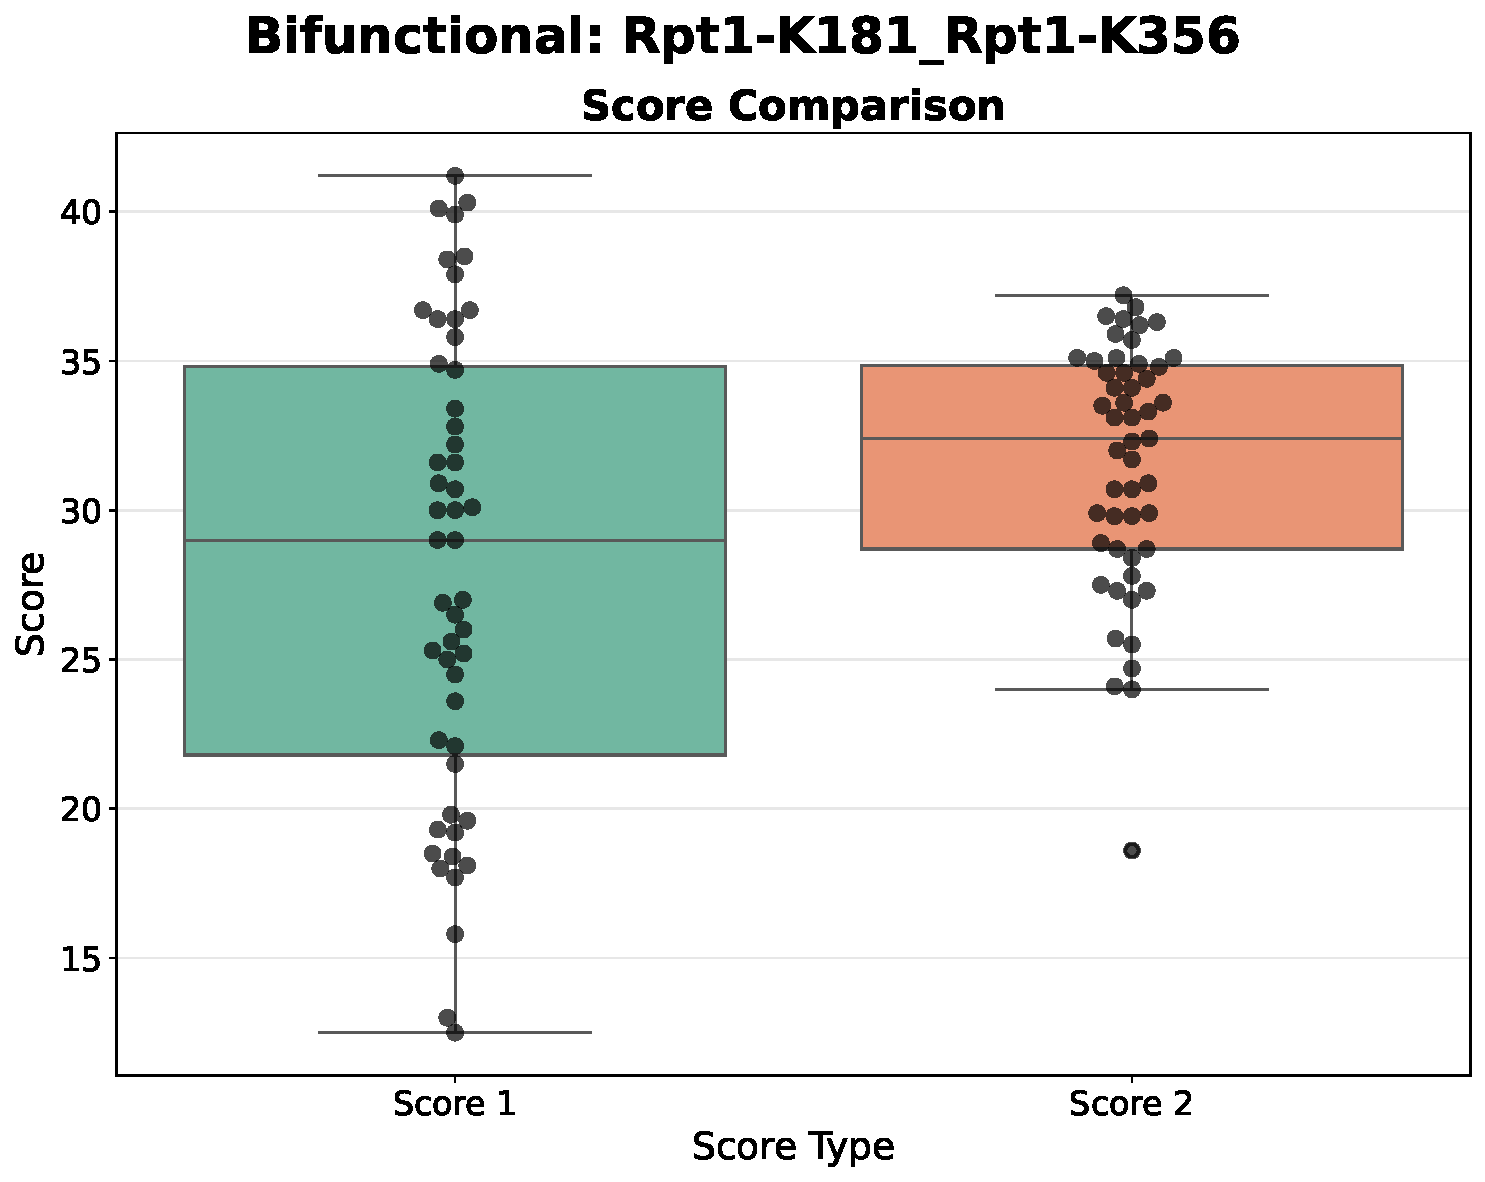
\includegraphics[width=\textwidth]{figures/bifunctional_score_freq.pdf}
        \caption{Raw ID score distribution}
    \end{subfigure}
    \hfill
    \begin{subfigure}[b]{0.45\textwidth}
        \centering
        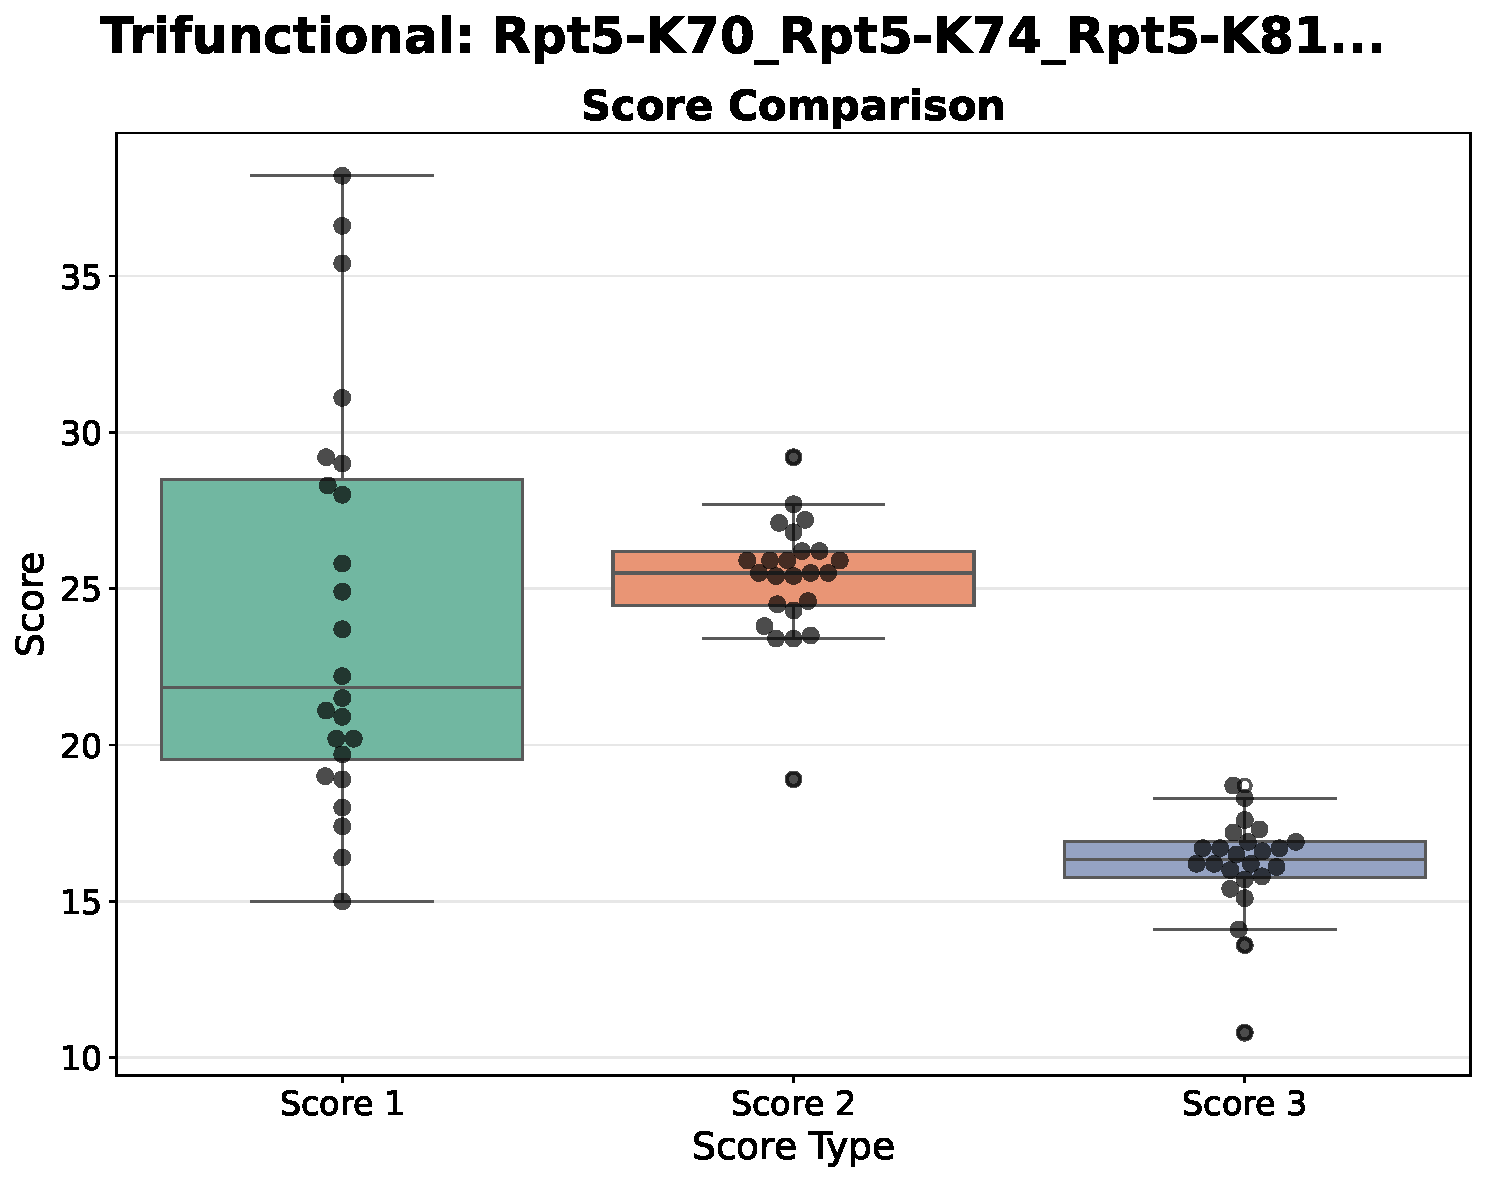
\includegraphics[width=\textwidth]{figures/trifunctional_score_freq.pdf}
        \caption{Normalized ID score distribution}
    \end{subfigure}
    \caption{Distributions of raw and normalized ID scores for trifunctional crosslinks.}
\end{figure}
\end{frame}

\begin{frame}{Noise model: extending Riccardo's bifunctional model to trifunctional crosslinks}
    
    \begin{columns}
    
        \begin{column}{0.45\textwidth}
            \begin{block}{1. Create "Ground Truth"}
                \begin{itemize}
                    \item Create 10,000 particles in a 3D box.
                    \item Define "True" geometry: A triplet (A,B,C) is satisfied if all distances ($d_{ab}, d_{ac}, d_{bc}$) are $< 25$ \AA.
                \end{itemize}
            \end{block}
            
            \begin{block}{2. Generate "Perfect" Data}
                \begin{itemize}
                    \item Find 140 triplets that satisfy the true geometry. These are our True Positives (TPs).
                \end{itemize}
            \end{block}
        \end{column}
    
        \begin{column}{0.45\textwidth}
            \begin{block}{3. Corrupt the Data (Add Noise)}
                \begin{itemize}
                    \item \textbf{Over-length TPs (28):} Take 20% of TPs and add noise to one distance, making it "too long" (e.g., $d_{bc}' = d_{bc} + \mathcal{N}(0, 10\AA)$).
                    \item \textbf{False Positives (60):} Add 60 completely random triplets.
                \end{itemize}
            \end{block}
            
            \begin{block}{4. Simulate ID Scores}
                \begin{itemize}
                    \item Assign \textbf{high scores} (e.g., 0.7-1.0) to all TPs (both good and over-length).
                    \item Assign \textbf{low scores} (e.g., 0.0-0.4) to all FPs.
                \end{itemize}
            \end{block}
        \end{column}
        
    \end{columns}

\end{frame}

\begin{frame}
    \frametitle{Forward model: Extension to trifunctional crosslinks}
    \begin{block}{}
        Forward model for bifunctional crosslinks 
        \begin{itemize}
            \item Consider the coordinates of coarse grained beads (residues) $\vec{r1}$ and $\vec{r2}$ connected by a bifunctional crosslinker.
            \item The uncertainty in the C$-\alpha$ atom position can be modeled using a sphere around the bead defined by $\sigma1$ and
            $\sigma2$ respectively.
            \item The distance between the centers of the spheres is $d = ||\vec{r1} - \vec{r2}||$.
            \item The probability that the crosslink is satisfied (i.e., the two residues are within the crosslinker length 
            $l_{xl}$) is to be computed, geometrically the problem is simplified as finding the volume of intersection of two spheres,
            the spheres representing the uncertainty in the position of the two residues        
        \end{itemize}

        \end{block}
\end{frame}
%----------------------------------------------------------------------------
\begin{frame}
\frametitle{Model problem}
\begin{figure}
    \centering
    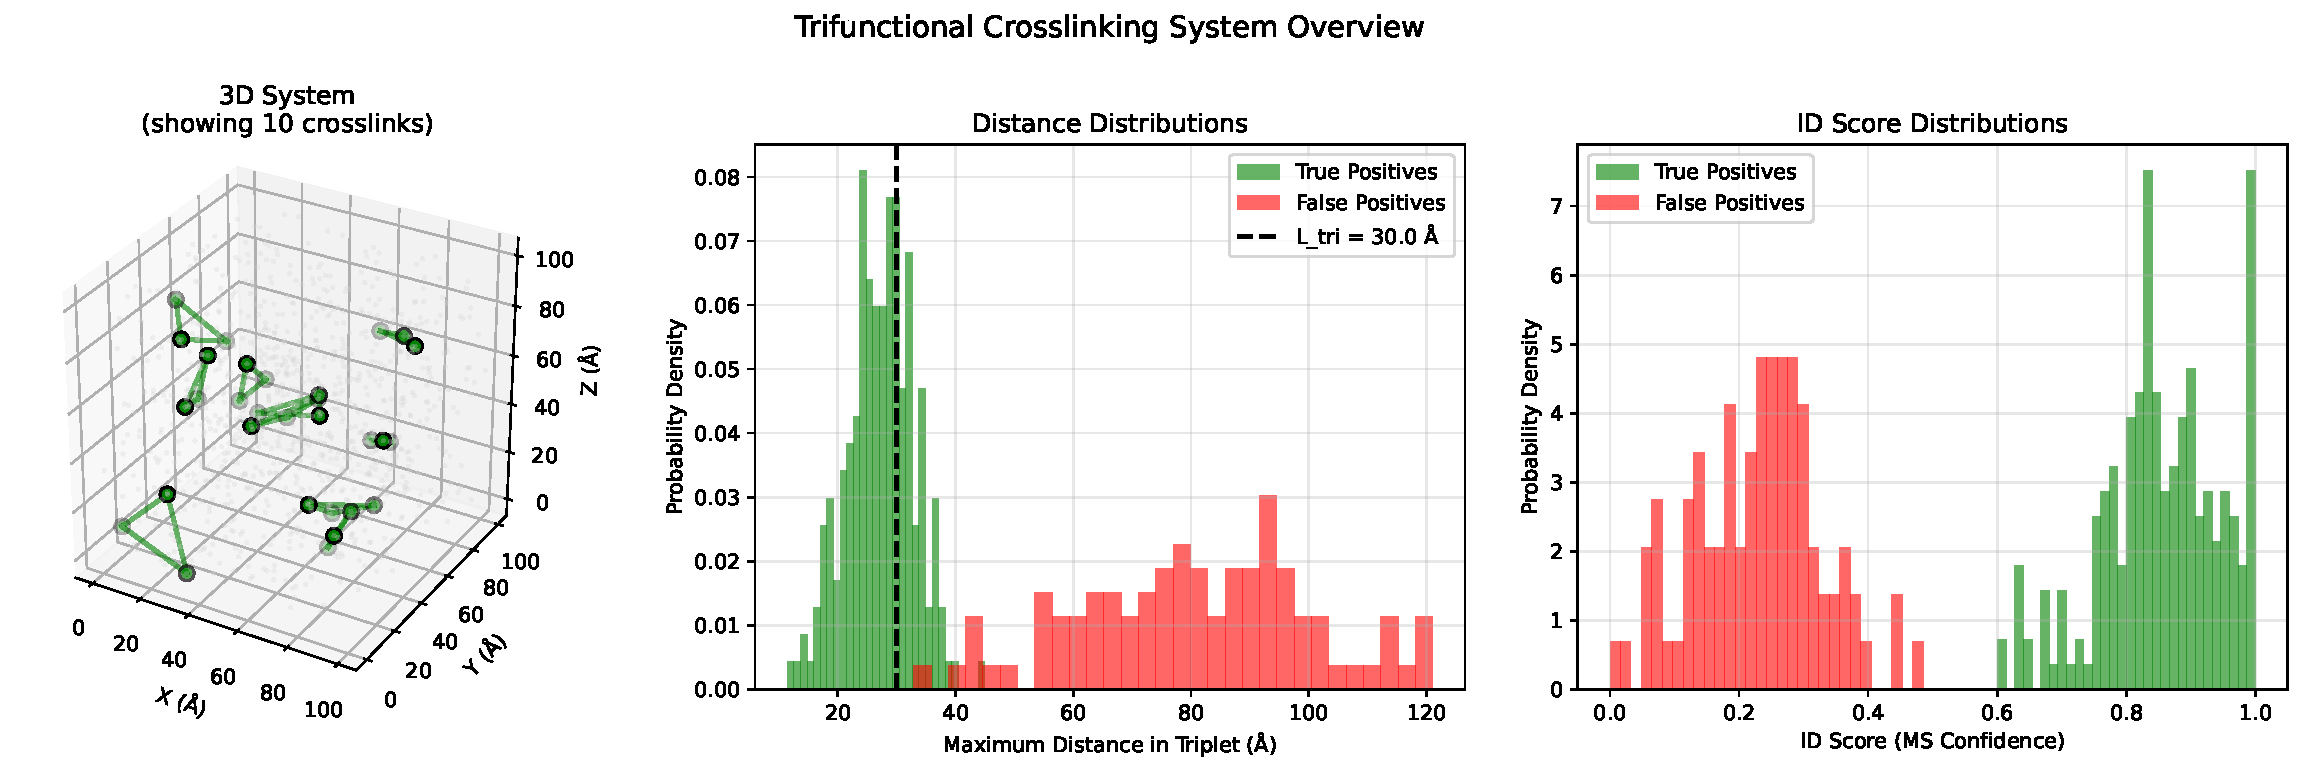
\includegraphics[width=0.6\textwidth]{figures/crosslinking_system.pdf}
    \caption{Schematic of the model problem setup}
\end{figure}
\end{frame}
%----------------------------------------------------------------------------
\end{document}
%**********************************************************************
